\chapter{Integration strategy}


\section{Entry criteria}
Before the integration testing phase proper may begin, it is important that the code has been inspected, manually or otherwise, and that unit tests have been run, so that any bug or issue found in this phase may be safely flagged as being a problem of integration and not something that works as it shouldn't at a lower level.


\section{Elements to be integrated}
\begin{figure}
\centering
\includegraphics[width=\textwidth]{tex-images/interactions}
\caption{The different architectural components and their interaction -- see the \emph{Design Document}}
\end{figure}
As detailed in the \emph{Design Document}, the architecture is organized in several higher level components themselves divided in lower level modules. In the integration phase it is important to test both the interaction between modules and that among components. Refer to the \emph{Design Document} itself for a detailed description of the elements. Follows here a list with a symbolic name, referred to in the schemes later on.

\subsection{Client Tier}
\subsubsection{Central Messenger}
\begin{itemize}
\item [A1] A module that interfaces with GUI;
\item [A2] A module that interfaces with GPS Reader;
\item [A3] A module that interfaces with Server Central Messenger;
\item [A4] A module that handles and forwards messages to modules.
\end{itemize}

\subsubsection{GPS Reader}
\begin{itemize}
\item [B1] A module that interfaces with Central Messenger in order to receive requests and send information;
\item [B2] A module that reads GPS information from Mobile APIs.
\end{itemize}

\subsubsection{Graphical User Interface}
\begin{itemize}
\item [C1] A module that interfaces with Central Messenger in order to receive and send messages;
\item [C2] A module that shows navigation pages.
\end{itemize}

\subsection{Web Tier}
\subsubsection{Central Messenger}
\begin{itemize}
\item [D1] A module that interfaces with Queue handler;
\item [D2] A module that interfaces with Request Allocator;
\item [D3] A module that interfaces with Request Gatherer;
\item [D4] A module that interfaces with Coverage Manager;
\item [D5] A module that interfaces with Sign Up/Log In manager;
\item [D6] A module that interfaces with Client Central Messenger;
\item [D7] A module that interfaces with Client Browser;
\item [D8] A module that handles and forward messages throw modules.
\end{itemize}


\subsection{Business Tier}
\subsubsection{Sign Up Manager}
\begin{itemize}
\item [E1] A \emph{Communication module} that interfaces with Central Messenger;
\item [E2] An \emph{Analysis module} that, reading form \emph{Data module}, analyses the correctness of data and it eventually confirms or rejects;
\item [E3] A \emph{Data module} that stores data in the correct database and read needed information.
\end{itemize}

\subsubsection{Log In Manager}
These modules perform exactly as the Sign Up Manager, so their functional integration testing is handled in the exact same way.
\begin{itemize}
\item [E1] A \emph{Communication module} that interfaces with Central Messenger:
\item [E2] An \emph{Analysis module} that, reading form \emph{Data module}, analyses the correctness of data and it eventually confirms or rejects;
\item [E3] A \emph{Data module} that stores data in the correct database and read needed information.
\end{itemize}

\subsubsection{Coverage Manager}
\begin{itemize}
\item [F1] A \emph{Data module} that interfaces with databases making DBMS queries;
\item [F2] An \emph{Analysis module} that analyses information received from \emph{Data module} and calculates the best coverage;
\item [F3] A \emph{Communication module} that interfaces with Central Messenger in order to send messages to Taxi Drivers selected by \emph{Analysis module}.
\end{itemize}

\subsubsection{Request Gatherer}
\begin{itemize}
\item [G1] A \emph{Communication module} that receives requests messages from Central Messenger;
\item [G2] An \emph{Analysis Module} that analyses data integrity and requests information received from \emph{Communication module} and eventually it sends to \emph{Data Module};
\item [G3] A \emph{Data Module} that stores information interfacing with databases.
\end{itemize}

\subsubsection{Request Allocator}
\begin{itemize}
\item [H1] A \emph{Data Module} that, periodically reading from databases, controls if there are requests to fulfil and updates taxi drivers’ information;
\item [H2] An \emph{Analysis module} that choses taxi diver to allocate to the requests;
\item [H3] A \emph{Communication module} that interfaces with Central Messenger in order to send notifications to taxi drivers.
\end{itemize}

\subsubsection{Queue Handler} 
\begin{itemize}
\item [I1] A \emph{Communication module} that receives availability messages from Central Messenger;
\item [I2] A \emph{Data module} that stores and updates information in database.
\end{itemize}


\section{Integration testing strategy}
Since, as stated, the high level components are divided in low level modules, it is at first necessary to test the integration of the modules that make a single component before that same component can be tested against the others at the higher level.

A top down approach will be followed for the integration of the components. The process is very much simplified by the almost complete independence of most of the different components.

For the integration test of the modules inside components we have chosen to use a \emph{Big Bang} approach that allows us to test the interaction between the modules of a specific component when they are all developed. We thought this was acceptable because of the small number of modules in each component. We also made this choice because in most cases modules are interfaces towards other components so their interaction is tested during integration test of components.


\section{Sequence of integration}

\subsection{Modules}
As stated, the chosen methodology is the \emph{Big Bang} approach, due to the small number of modules each component is made of. Therefore, no explicit sequence is given for their integration.

\begin{figure}
\centering
\includegraphics[width=\textwidth]{tex-images/mod-1}
\caption{Integration testing in modules of the App Central Messenger component}
\end{figure}

\begin{figure}
\centering
\includegraphics[width=0.5\textwidth]{tex-images/mod-2}
\caption{Integration testing in modules of the App GPS Reader component}
\end{figure}

\begin{figure}
\centering
\includegraphics[width=0.5\textwidth]{tex-images/mod-3}
\caption{Integration testing in modules of the App Graphical User Interface component}
\end{figure}

\begin{figure}
\centering
\includegraphics[width=\textwidth]{tex-images/mod-4}
\caption{Integration testing in modules of the Server Central Messenger component}
\end{figure}

\begin{figure}
\centering
\includegraphics[width=0.5\textwidth]{tex-images/mod-5}
\caption{Integration testing in modules of the Server Sign-Up Manager and Log-In Manager components}
\end{figure}

\begin{figure}
\centering
\includegraphics[width=0.5\textwidth]{tex-images/mod-6}
\caption{Integration testing in modules of the Server Coverage Manager component}
\end{figure}

\begin{figure}
\centering
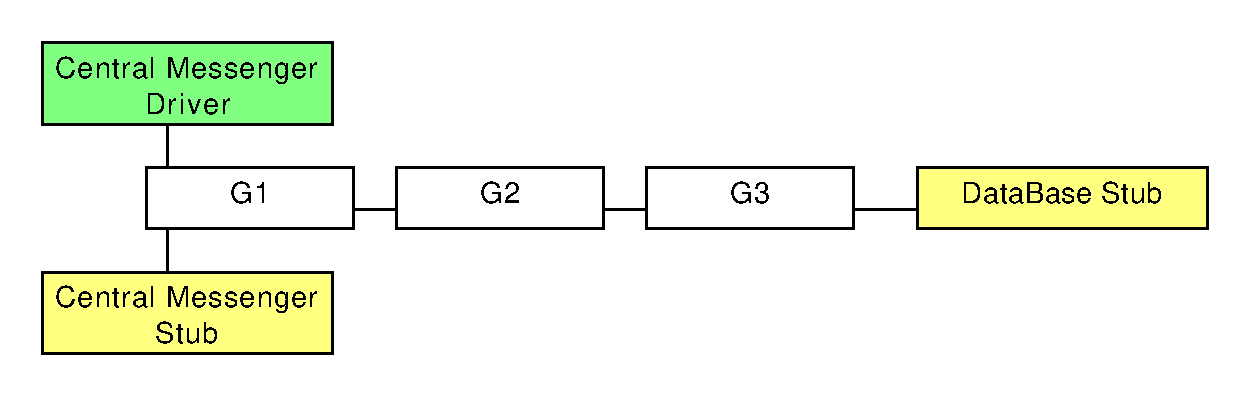
\includegraphics[width=0.5\textwidth]{tex-images/mod-7}
\caption{Integration testing in modules of the Server Coverage Manager component}
\end{figure}

\begin{figure}
\centering
\includegraphics[width=0.5\textwidth]{tex-images/mod-8}
\caption{Integration testing in modules of the Server Request Allocator component}
\end{figure}

\begin{figure}
\centering
\includegraphics[width=0.5\textwidth]{tex-images/mod-9}
\caption{Integration testing in modules of the Server Queue Handler component}
\end{figure}

\clearpage
\subsection{Components}
Since a top down (from the user interface) approach will be used, the integration order will be as follow:
\begin{enumerate}
\item Client App GUI;
\item Client App Messenger;
\item Client App GPS Reader;
\item Client Webapp (on par with the three previous components);
\item Central messenger;
\item Log in manager;
\item Sign up magager;
\item Request allocator;
\item Coverage manager;
\item Queue handler;
\item Request gatherer;
\item All Database Management Systems.
\end{enumerate}

\begin{figure}
\centering
\includegraphics[width=\textwidth]{tex-images/comp-1}
\caption{First step in integration testing for components}
\end{figure}

\begin{figure}
\centering
\includegraphics[width=\textwidth]{tex-images/comp-2}
\caption{Second step in integration testing for components}
\end{figure}

\begin{figure}
\centering
\includegraphics[width=\textwidth]{tex-images/comp-3}
\caption{Third step in integration testing for components}
\end{figure}

\begin{figure}
\centering
\includegraphics[width=\textwidth]{tex-images/comp-4}
\caption{Fourth step in integration testing for components}
\end{figure}

\begin{figure}
\centering
\includegraphics[width=\textwidth]{tex-images/comp-5}
\caption{Fifth step in integration testing for components}
\end{figure}

\begin{figure}
\centering
\includegraphics[width=\textwidth]{tex-images/comp-6}
\caption{Sixth step in integration testing for components}
\end{figure}

\begin{figure}
\centering
\includegraphics[width=\textwidth]{tex-images/comp-7}
\caption{Seventh step in integration testing for components}
\end{figure}

\begin{figure}
\centering
\includegraphics[width=\textwidth]{tex-images/comp-8}
\caption{Eighth step in integration testing for components}
\end{figure}

\begin{figure}
\centering
\includegraphics[width=\textwidth]{tex-images/comp-9}
\caption{Ninth step in integration testing for components}
\end{figure}

\begin{figure}
\centering
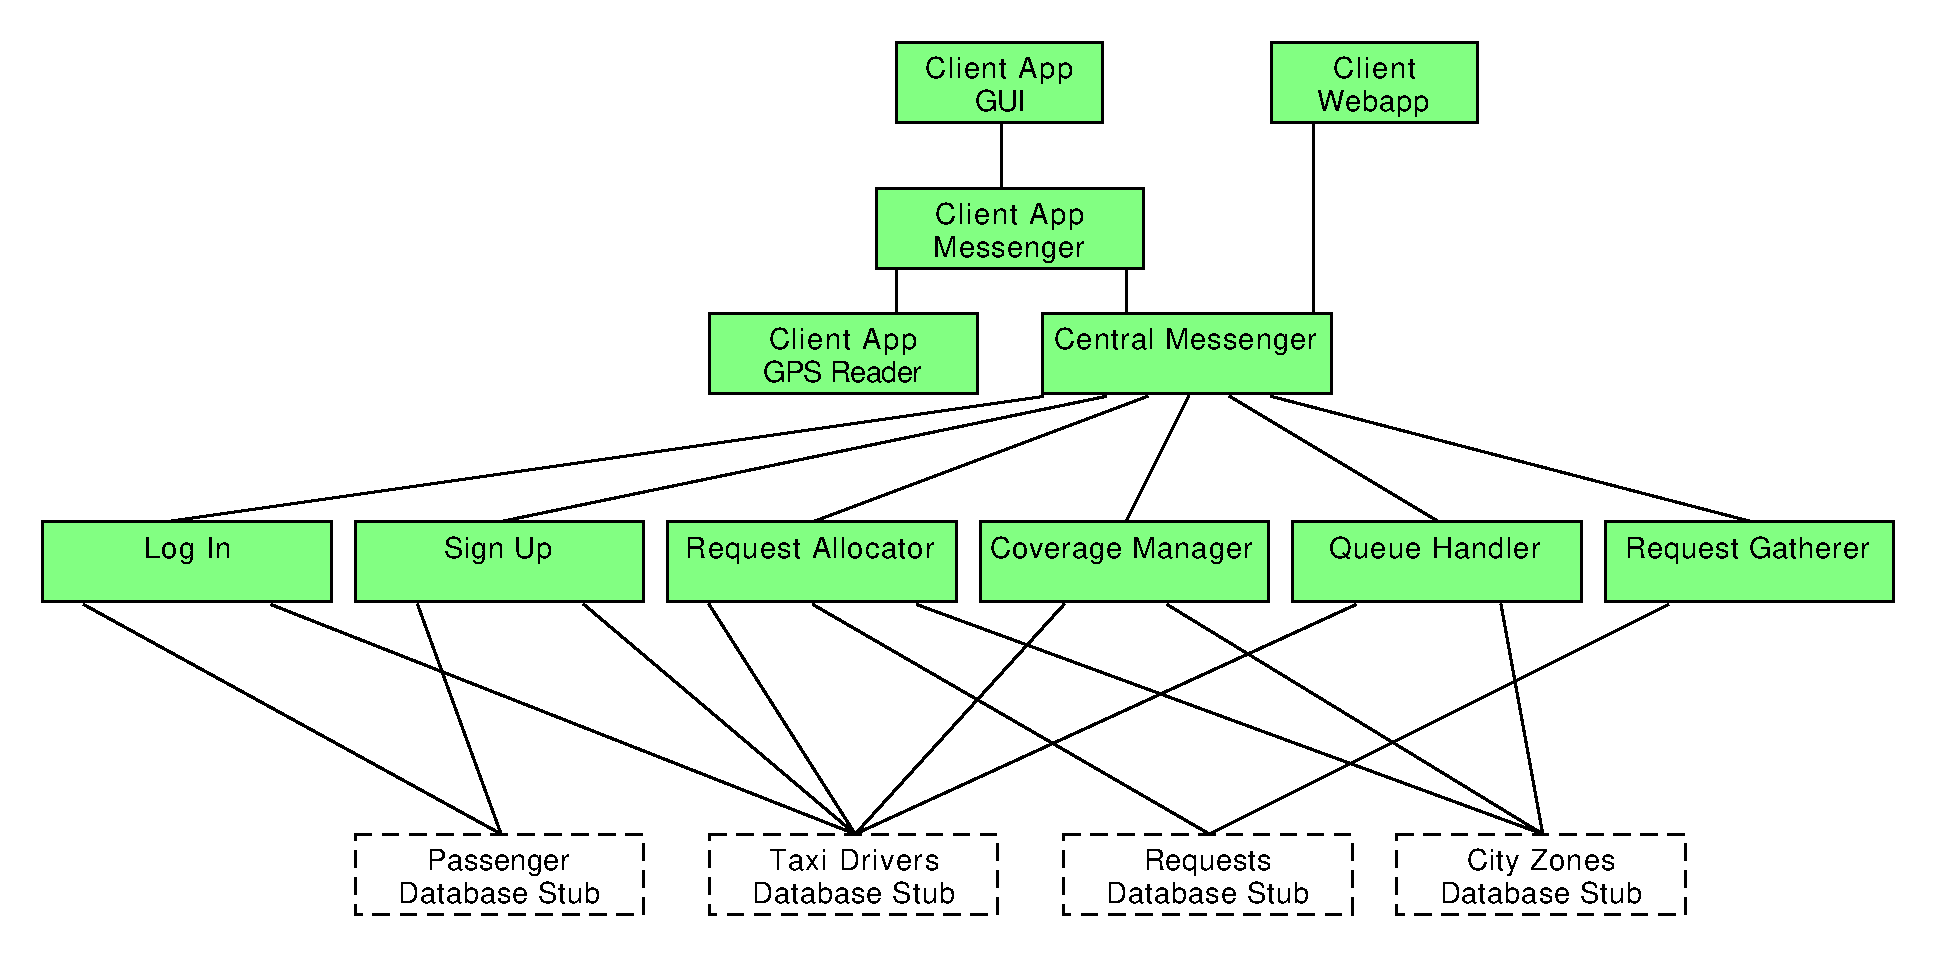
\includegraphics[width=\textwidth]{tex-images/comp-10}
\caption{Tenth step in integration testing for components}
\end{figure}

\begin{figure}
\centering
\includegraphics[width=\textwidth]{tex-images/comp-11}
\caption{Final step in integration testing for components: all components integrated}
\end{figure}
